%%% Local Variables:
%%% mode: latex
%%% TeX-command-extra-options: "-shell-escape"
%%% TeX-master: t
%%% End:

%%% Preamble
\documentclass[paper=a4, fontsize=11pt]{report}
\usepackage[utf8]{inputenc}  
\usepackage[T1]{fontenc}
\usepackage{fourier}
\usepackage[english]{babel}															% English language/hyphenation
\usepackage[protrusion=true,expansion=true]{microtype}	
\usepackage{amsmath,amsfonts,amsthm} % Math packages
\usepackage[pdftex]{graphicx}	
\usepackage{url}
\usepackage{tikz}
\usepackage{pdftexcmds}
\usepackage{minted}

%%% Custom sectioning
\usepackage{sectsty}
\allsectionsfont{\centering \normalfont\scshape}

%%% Custom headers/footers (fancyhdr package)
\usepackage{fancyhdr}
\pagestyle{fancyplain}
\fancyhead{}											% No page header
\fancyfoot[L]{}											% Empty 
\fancyfoot[C]{}											% Empty
\fancyfoot[R]{\thepage}									% Pagenumbering
\renewcommand{\headrulewidth}{0pt}			% Remove header underlines
\renewcommand{\footrulewidth}{0pt}				% Remove footer underlines
\setlength{\headheight}{13.6pt}


%%% Equation and float numbering
\numberwithin{equation}{section}		% Equationnumbering: section.eq#
\numberwithin{figure}{section}			% Figurenumbering: section.fig#
\numberwithin{table}{section}				% Tablenumbering: section.tab#


%%% Maketitle metadata
\newcommand{\horrule}[1]{\rule{\linewidth}{#1}} 	% Horizontal rule
\newcommand{\espr}[1]{
  \mathrm{E}^Q \left[ #1 \right]
}

\newcommand{\Qespr}[2]{
  \mathrm{E}^{#1} \left[ #2 \right]
}


\title{
		%\vspace{-1in} 	
		\usefont{OT1}{bch}{b}{n}
		\normalfont \normalsize \textsc{Ecole Polytechnique} \\ [25pt]
		\horrule{0.5pt} \\[0.4cm]
		\huge Modèles des Taux d'interêt \\
		\horrule{2pt} \\[0.5cm]
}
\author{
		\normalfont \normalsize
                Bachir EL KHADIR\\[-3pt] \normalsize
                \today	
}
\date{}

\theoremstyle{definition}
\newtheorem{theorem}{Theorem}
\newtheorem{defn}{Definition}

\newcommand{\IMG}[3]{
  \begin{center}
    \includegraphics[scale=#3]{#1}%
    \end{center}
}


%%% Begin document
\begin{document}
\maketitle

\newpage
\tableofcontents



%%% Local Variables:
%%% mode: latex
%%% TeX-master: "main.tex"
%%% End:

\section{Remerciments}

Ecole Polytechnique
Maitre de stage
Bla bla bla


%%% Local Variables:
%%% mode: latex
%%% TeX-master: "main"
%%% End:

\newpage

\subsection*{Résumé}
  
  Ce rapport présente quelques outils utilisés lors du pricing de dérivés de taux. 
  Il est particulièrement centré sur le modèle de Hull White qui est conduit par deux facteurs (appelé aussi G2++).  J'adopterai le plan suivant dans la rédaction de ce rapport:
  \begin{itemize}
  \item 
    La première partie introduit le marché de taux par un certain nombre de définitions qui lui sont propres, ainsi que les produits financiers principaux utilisés pour la calibration des modèles.
  \item 
    Dans la deuxième partie je présenterai quelques modèles existant, et je discuterai de leurs limites et de leurs implémentions pratique.
  
  \item
    La troisième partie présente les résultats concrets que j'ai obtenus dans le cas du modèle gaussien à deux facteurs, ainsi que la partie calibration de modèle.
  \end{itemize}
  
\subsection*{Abstract} 
This report presents some tools used in the pricing of intereset rates derivatives. It's focused on two factors Hull-White model (called G2++).  
  \begin{itemize}
  \item
    The first part introduces some definitions relative to the interest rates market, as well as some derivative used later in the calibration.
  \item
    In the second part I will present some existing models, their limitations and possible implementation.

  \item
    The last part presents the results I obtained using the G2++ model and the calibration process.
  \end{itemize}




\newpage
\chapter*{Introduction}

J'ai fait mon stage a JP Morgan équipe exotic rates. La plus grosse partie du travail consistait à trouver le bon modèle mathématique pour pricer un produit et le calibrer au marché.

L'intérêt que porte les banques aux produits exotiques a considérablement augmenté au cours des dernières années. Plusieurs modèles ont été développé pour refléter au mieux le comportement des marchés financiers.

Le département au sein duquel j'ai effectué mon stage s'occupait des produits basé sur les taux d'intérêt. Dans ce domaine, une propriété appréciable dans un modèle est le fait qu'il possède un nombre de paramètres suffisant pour être calibré parfaitement aux prix observables dans la réalité, sans pour autant ``overfitter'' l'échantillon disponible, surtout que dernièrement, depuis la crise des subprimes, le marché des taux a connu des changement radicaux que les modèles traditionnels n'arrive pas décrire. La possibilité d'observer des taux négatifs en est un exemple. 

Un produit en particulier n'a cessé de  gagner en notoriété: les cancelables spread options. Ma mission de stage était de comprendre les modèles existant et leurs implémentations qui permettent de pricer (entre autres) ce type de produits, comprendre leurs limites, et essayer de trouver des améliorations.

Ce stage est à forte composante informatique, une attention particulière a été accordée aux détails d'implémentation et optimisation du code.
 

%%% Local Variables:
%%% mode: latex
%%% TeX-master: "main"
%%% End:


\chapter{Préliminaires sur les taux d'interêts}

\section{Définiton}
\begin{defn}
On dénote le prix de zéro coupon forwardé $P(T, S)$ le montant qu'il faut investir à dans un instrument risque-neutre au temps $T$ pour obtenir une unité de monnaie au temps $S$.
\end{defn}

\begin{defn}
On définit $f(t, T)$ le taux d'intêret instantané forwad à la date $t$ pour une maturité $T$ la quantité $$f(t, T) := - \frac{ \delta}{\delta T}  log P(T, S)$$
\end{defn}

\begin{defn} Le taux instantanné est défini par
  $r_t = \underset{T \to t}{lim}f(t, T) $ \\
  Le taux d'actualisation (stochastique) est: $D_t^T := e^{-\int_t^Tr_s \rm{d}s}$
\end{defn}

\iffalse
\begin{defn}
  Le taux d'interet cumulé entre deux période $t$ et $T$ est la quantité $R(t, T)$ que $r_t$ doit égaler spour avoir le même rendement
\end{defn}
\fi

\begin{defn}
  Le taux d'interet forward $F(t; T, S)$ est la prévision  à l'instant $t$ du taux entre deux période $T$ et $S$.
  Ce taux est la quantité $L$ connu à l'instant qui annule la valeur de ce contrat à l'instant $t$:
  \begin{itemize}
  \item Recevoir l'interêt  $L$ sur un 1 euro entre $T$ et $S$
  \item Payer le taux variable  $F(T, S)$ sur un 1 euro entre $T$ et $S$
  \end{itemize}
\end{defn}


le taux $r_t$ n’est pas un produit échangé sur le marché que l’on peut mettre en portefeuille. On ne peut donc pas construire de couverture d’un produit donné de la même manière que dans un modèle d’action, et ce malgré la similitude des modèles mathématiques.

\section{Mesures équivalentes}

Nous nous plaçons dans le cadre d'une économie à temps continu, qui admet une espace de probabilité $(\Omega, \cal{F}, \mathbb{P})$, avec $K+1$ actifs tradables, que nous appelerons actifs de base, dont le prix est donné par $(S_t = (S^0_t, ...S^k_t))_{t \geq 0}$. Dans toute la suite nous confondons l'actif et son prix.
$S^0$ étant l'actif sans risque, qui évolue donc au temps sans risque $$\mathrm{d}S^0_t = r_t S^0_t \mathrm{d}t$$
ie $$S^0_t = e^{-\int_0^t r_s \mathrm{d}s}$$

Par définition, nous connaissons le prix des actifs $K+1$, dans la prochaine section nous détaillerons la procédure de pricing de produits plus compliqués.

\subsubsection{Principe de pricing}
A travers les $K+1$ actifs de base, nous construisons des produits plus complexes. 
Le prix de ce dernier est donc intimement lié à la possibilité de trouver une stratégie auto-financée qui le réplique.
Commençons d'abord par définir ce qu'est une stratégie auto financé.

\begin{defn}
  \begin{itemize}
  \item Une stratégie est une processus $(\Phi_t = (\Phi^0_t, ... \Phi^K_t))_t$ localement borné et adapté à la filtration $\cal{F}$.
  \item La valeur associé à cette stratégie est donné par $V_t(\Phi) = <\Phi_t, S_t>$.
  \item Une stratégie est auto financée sir $\mathrm{d}V_t = \Phi_t \mathrm{d}S_t$
  \end{itemize}
\end{defn}

Une hypothèse souvent utilisée dans le cadre de la finance de marché est l'abscence d'abitrage. Une opportunité d'arbitrage est la possiblité d'investir 0 aujourd'hui, et recevoir, avec probabilité non nulle, un montant positive dans le future. En d'autres termes, l'abscence d'arbitrage signifie que si $\Phi$ est une stratégie auto financée telle que $V_0(\Phi) = 0$, alors $\mathbb{P} ( V_t(\Phi) > 0 ) = 0$. Ceci nous permettra de valoriser des produits complexes en répliquant leur payoff par une combinaison linéaire de produits simple dont le prix est connue.

Une deuxième hypothèse que nous admettrons dans la suite est la complétude du marché: Tout les produits utilisés seront consiédérés disponible à tout moment et en quantité abandante (liquide), ie à chaque instant $t$, pour tout payoff $H$, il existe une stratégie autofinancée associée $\Phi$ qui vérifie $V_t( \Phi ) = H$. Nous ne traiterons pas le cas des produits illiquide. Ceci est justifié, le marché des taux étant l'un des plus gros en volume dans le monde.

Nous pouvons montrer(*) que ces hypothèse sont équivalent à l'existence d'une mesure de probabilité risque neutre $Q$ unique sous laquelle le prix actualisé de tous les produits tradables sont des martingales. ie si un on note $H_t$ le prix à l'instant $t$ d'un produit financier, alors
$$H_t =\espr{ \frac{H_s}{S^0_t} | F_t } = V_t(\Phi)$$

En particuler, le prix d'un zéro coupon qui paye 1 à l'instant $T$ est donné par
$$ P(t, T) := \espr{  e^{-\int_t^T r} } $$


Nous pouvons interpréter le ratio $\frac{H_s}{ S^0_s}$ comme étant le nombre  de $H$ par unité de discount factor stochastique $S^0$. Le discount factor est appelé dans ce cas numéraire. Nous verrons maintenant que nous pouvons choisir un autre numéraire plus adapté au produit que nous voulons pricer.
En effet le changement de numéraire préserve la propriété d'autofinancement d'un portefeuille.

\begin{defn} Un numéraire est tout actif financier ne payant pas de dividendes \end{defn}

\begin{defn} Mesure de probabilité équivalente.
  
Supposons qu’il existe un numéraire $(M_t )_{t \geq 0}$ et une mesure martingale équivalente $Q^M$ telle que le prix de chaque actif actualisé par le processus M soit une$Q_M$-martingale. 
$$ \frac{S^i_t}{M_t} = \Qespr{Q^M}{ \frac{S^i_T}{M_T} | F_t}$$
Soit $(N_t )_{t \geq 0}$ un numéraire. \\
Alors il existe une mesure de probabilité $Q_N$ telle que le prix de chaque actif actualisé par le processus $N$ soit une $Q_N$-martingale, i.e.
$$ \frac{S^i_t}{N_t} = \Qespr{Q^N}{ \frac{S^i_T}{N_T} | F_t}$$

où $Q^N$ est définie par:
$$\Qespr{Q^N}{ H } = \Qespr{Q^M}{ \frac{ M_T/N_T}{M_0/N_0} H}$$

\end{defn}

Example: Mesure forward neutre

Le bond zéron coupon dont la maturité concide avec la date du payment d'un produit financier peut servir de numéraire. Nous appellerons la mesure de probabilité associé $Q_T$.

Dans ce cas $P(T, T) = 1$, et par conséquent il suffit de calculer l'espérance du payoff (divisé par 1) sous $Q_T$.
Si nous notons le payoff de ce produit $H$, alors son prix à l'instant $0$ est donné par $$P(t, T) \, \Qespr{Q_T}{ H | F_t } $$
Pour que celà nous soit utile, il faut que la dynamique de $H$ soit connue sous $Q_T$. Ceci est vérifié pour les contrats payant un taux d'interêt sur un nominal fixe. En effet $(F(t; S, T))_t$ est une martingale 
$$ \Qespr{Q_T}{ F(t; S, T) | F_u } = F(u; S, T)$$

\textbf{Preuve:}
Si nous disposons de  $\frac{P(t, S)}{(1+(T-S)F(t; S, T))}$ au temps $t$, nous pouvons acheter $\frac{1}{(1+(T-S)F(t; S, T))}$ unités de l'obiligation $P(t, S)$, nous obtenons $\frac{1}{(1+(T-S)F(t; S, T))}$ au temps $S$, cette somme là est, par définition de $F$, équivalente à l'obtention de 1 à l'instant $T$, qui exactement le payoff de l'obligation $P(t, T)$.
Par principe de \textbf{non arbitrage}, ces deux investissement doivent avoir le même coût, ie:
$ \frac{1}{T-S} \left( \frac{P(t, S)}{P(t, T)} - 1  \right) $
La preuve en découle.

\newpage

\section{Produits financier d'interêts}

Le dévelopement de la section précédente nous sera utile pour pricer les dériver des taux.
Considérons le cas particlier d'un call eurpéen à maturité $T$, strike $K$, dont le sous-jacent est bond zéro coupon qui expire à l'instant $S$. Le payoff d'un tel contrat est connu: $ (P(T, S) - K)^+)$. Son prix à un instant antérieur $t$ est
$$ZBC(t, T, S, K) := \espr{ e^{-\int_t^T r_s \rm{d}s} \, (P(T, S) - K)^+ | F_t }$$
Il est plus pratique de considérer la forward mesure, sous laquelle le prix du call s'écrit
$$ZBC(t, T, S, K) = P(t, T) \, \Qespr{Q_T}{(P(T, S) - K)^+ | F_t}$$
De même, pour un put
$$ZBP(t, T, S, K) = P(t, T) \, \Qespr{Q_T}{(K - P(T, S))^+ | F_t}$$

Cette écriture nous rappelle la formule de blackscholes pour les options sur les actions.

\begin{defn}
  Swap:
Un swap est un contract entre deux parties qui s'engagent à échanger des flux financiers pendant une durée et à une fréquence détérminées. la plupart du temps, ces flux sont détérminé comme étant l'intêret à un taux fixe $K$ contre un taux variable (LIBOR ${L(T_i)}_i$ par examplesur un notionnel $N$. 
$$ N \sum D_t^{T_i} \tau_i (L(T_{i-1}) - K) $$
\end{defn}


\begin{defn}
  Caplet/floorlet:
  Un caplet/floorlet peut être vu comme un call/put européenne sur un
  Son payoff est le suivant
$$ \tau (L(T, S) - K)^+ $$
\end{defn}

\begin{align}
  Cpl(t, T, S, \tau, X)
  &= \espr{ e^{-\int_t^S r_s \rm{d}s} \tau (L(T, S) - K)^+ | F_t} \\ 
  &= \espr{ e^{-\int_T^S r_s \rm{d}s} P(t, T)  \tau (L(T, S) - K)^+ | F_t} \\
  &= \espr{ e^{-\int_T^S r_s \rm{d}s} (1 - (1 + X \tau)P(t, T))^+ | F_t} \\
  &= (1 + X \tau) \espr{ e^{-\int_T^S r_s \rm{d}s} (\frac{1}{1 + X \tau} - P(t, T))^+ | F_t} \\
  &= (1+X \tau) ZBP(t, T, S, \frac{1}{1+X \tau})
\end{align}

\begin{defn}
  Cap/floor:
Un cap/floorlet peut être vu comme une somme de caplets
$$ N \sum D_t^{T_i} \tau_i (L(T_{i-1}) - K)^+ $$
\end{defn}

La forme des payoff indique que le cap permet de protéger son détenteur d’une hausse des taux Libor, et symétriquement que le floor protège d’une éventuelle baisse de ces taux.


%%% Local Variables:
%%% mode: latex
%%% TeX-master: "main"
%%% End:

%%% Local Variables:
%%% mode: latex
%%% TeX-master: "main"
%%% End:

\chapter{Les différents modèles des taux d'interêts}

Nous avons vu dans la partie précédente que pour trouver le prix des dérivés de taux et pouvoir calculer l'espérance, il faut donner la dynamique qui régit le sous-jacent, dans notre cas  $r_t$.

Les professionnels des marchés de taux ont prix l'habitude d'évaluer les options vanille avec la formule de Black \& Scholes. Ils font l'hypothès implicite que les taux Libor $L(t, T)$ forward sont log normaux dans la mesure forward associée à leur échéance:
$$\mathrm{d} L_t(T, S) = \sigma L_t(T, S) \mathrm{d}W_t$$
Ce modèle spécifie la dynamqieu de chaque taux Libor sous sa mesure forward associées. Cependat, il est indispensable d'un point de vue pratique de pouvoir exprimer les taux Libor forward sous une même mesure. 

Diffuser des taux Libor de différentes maturitées sous une même mesure forward peut introduire des distorsions lors du traitement numéerique. En effet, les  équation montrent que plus la maturité de la mesure utilisée pour diffuser un taux Libor forward est  éloignée de $T_i$, plus le terme de tendance est important, et par conséquent plus l’erreur numérique due à une approximation pour calculer cette tendance risque d’être importante.

L'aproche historique, décrit la dynamique du taux d'interêt instantané comme étant conduite par un driver à une seule dimension. Ceci est pratique dans le sens où les prix de zéro coupon et le taux sont directement disponible dans le modèle.
De plus, certains produits financiers dépendent directement la courbe de rendement.
Nous verrons que la donnée du taux instantané $r_t$ permet de caractériser complètement courbe de taux.

Il est important que la dynamique de $r_t$ soit à la fois riche pour pouvoir décrire la courbe de rendement observée dans le marché, et suffisemment simple pour que le temps nécessaire pour le calcul ne soit trop long. Le modèle de Hull White a été introduit en 1990.
$$ \mathrm{d}r_t =  (\theta(t) - \beta(t) r_t) \mathrm{d}t + \sigma(t) \mathrm{d} W_t$$

Un des atouts majeure de ce modèle est la possiblité de simuler la dynamique de $r_t$ par un arbre. Ceci étant essentiel pour pricer des produits qui dépendent de toute une partie de la courbe de taux, et non seulement d'un point précis. Les bermuda options en sont un exemple.

\section{Le modèle à deux facteurs}
\subsection{Motivation}

Considérons un produit $E$ dont le payoff  dépent  du spread entre un taux d'intêret cumulé entre $0$ et $T_1$ pour le premier et $0$ et $T_2$ pour le second. $E$ dépend donc de la distribution jointe des deux taux.

Dans la réalité, on observe sur les marchés que les taux à différentes maturités ne sont pas corrélés. Si on regarde le taux 2Y et 10Y

\IMG{img/libor.png}{Libor}{1}


La figure suivante, tiré cours \cite{Central} reproduit une matrice de corrélation par terme de variations quotidiennes de taux zéro-coupon. Il apparait très clairement que des taux de maturités proches, comme le taux de maturité 3 ans et celui de maturité 4 ans, sont très corrélés, tandis que des taux de maturité éloignées (par exemple le taux 1 mois et le taux 10 ans) le sont très peu:

\IMG{img/tabcorr.png}{Tableau de correlation}{0.3}


\subsection{Limite des modèle à un seul facteur}
Montrons dans un premier temps pourquoi un modèle à un seul facteur n'est pas suffisant pour pricer ces produits qui dépendent non seulement de la distribution de chaque courbe de taux, mais aussi de leur corrélation. 

Rappelons la dynamique de $r_t$ dans le cadre de Hull White:
$$r_t = k(\theta - r_t)  \mathrm{d}t  + \sigma \mathrm{d}W_t$$
La formule analytique de l'obligation zéro coupon est donc
$$P(t, T) = A(t, T) exp(-B(t, T) r_t)$$
En particulier le taux d'intêret cumulé est une donné par une transformation affine du taux instantané:
$$R(t, T) = \frac{ln P(t, T)}{T-t} =: a(t, T) + b(t, T) r_t$$
Le payoff du produit $E$ est donc fonction de la distribution jointe de $R(0, T_1)$ et $R(0, T_2)$. Sauf que:
$$Cor(R(0, T_1), R(0, T_2) = 1$$

On en déduit qu'un choc à $r_t$ agit de la même manière sur toutes les courbes.


Un modèle à un seul facteur ne capture pas ce comportement. Essayons de pallier à ce problème en rajoutons un facteur à ce modèle.

Dans cette section nous considérons un modèle où le taux d'intêret instantanté est donné par une somme de deux facteurs gaussiens centrés et corrélés. Dans ce modèle doit sa popularité au fait que le prix des obligations zéron coupon admet une formule exact, ainsi que le prix des caps et des floors.


\begin{align*}
  \rm{d}x &= -\beta^y x(t) \rm{d}t + \sigma^x \rm{d}W^x_t \\
  \rm{d}y &= -\beta^y y(t) \rm{d}t + \sigma^y \rm{d}W^y_t \\
  \rm{d}r &= x + y
\end{align*}


\section{Approximation de la solution par un arbre binomial}


L'équation (*) s'intègre simplement en:
$$x(t) = x(s) e^{-\beta^y (t-s)} +  \sigma^x \int_s^t e^{- \beta^y (t-u)} \rm{d} W^x_u $$
$$y(t) = x(s) e^{-\beta^y (t-s)} +  \sigma^y \int_s^t e^{- \beta^y (t-u)} \rm{d} W^y_u $$

\subsection*{Construction}

Cette méthode a été d'abord suggéré par Hull-White (1994)

On discrétise l’intervalle $[0, T]$ avec les temps $T_i = i \Delta t$, où $\Delta t = \frac{T}{N}$.
Nous donnons une approximation de la dynamique processus $x$ et $y$, par une suite de variable de discretisé $((\widetilde{x}_i, \widetilde{y}_i) \approx (x(i \Delta i), (y(i \Delta t))_i $. Pour celà nous calculerons les deux premier moment de $(x, y)$.

Nous faisons le calcul pour $x$, la même formule s'appliquera à $y$.
$$E(x(t+\Delta t) | F_t) = x(t) e^{-a \Delta t}$$
$$V(x(t+\Delta t) | F_t) = \frac{{\sigma^x}^2}{2a} (1 - e^{-2a \Delta t})$$
$$Cov\{x(t+\Delta t), y(t+\Delta t) | F_t \} = \frac{\sigma^x \sigma^y \rho}{a + b} (1-e^{-(a+b)\Delta t})$$

Pour que le $((\widetilde{x}_i, \widetilde{y}_i)$ et $(x(i \Delta i), (y(i \Delta t))_i $ aient les même moment, la loi de  $((\widetilde{x}_i, \widetilde{y}_i)$  est donnée par:
$$\mathrm{P} \left( \widetilde{x}_{i+1} = \widetilde{x}_i + a \, \mathrm{d}x, \widetilde{y}_{i+1} = \widetilde{y}_i + b \, \mathrm{d}y |  \widetilde{x}_i, \widetilde{y}_i \right) = p^{a, b}( \widetilde{x}_i, \widetilde{y}_i)$$
où 
\begin{itemize}
\item $a, b \in \{-1, +1\}$
\item $p$ est donnée par:
$$ p^{a, b}(x, y) = \frac{1 + a \rho}{4} - b \frac{\beta^y \sigma^x y + a \sigma^x \sigma^y  x}{4 \sigma^x \sigma^y} \sqrt{\Delta t} $$
\end{itemize}

Le schéma suivant résume les transitions du processus {$(\widetilde{x}, \widetilde{y})$};
%%% Local Variables:
%%% mode: latex
%%% TeX-master: "main.tex"
%%% End:

\tikzstyle{bag} = [text width=10em, text centered]
\tikzstyle{end} = []
\begin{figure}[h!]
  \centering
\begin{tikzpicture}[sloped]
  \node (xy) at (0,0) [bag] {$(\widetilde{x}, \widetilde{y})$};
  \node (a) at ( 3,-2) [bag] {$(\widetilde{x} + \rm{d}x, \widetilde{y} + \rm{d}y)$};
  \node (b) at ( -3,-2) [bag] {$(\widetilde{x} + \rm{d}x, \widetilde{y} - \rm{d}y)$};
  \node (c) at ( 3,2) [bag]{$(\widetilde{x} - \rm{d}x, \widetilde{y} + \rm{d}y)$};
  \node (d) at ( -3,2) [bag]{$(\widetilde{x} - \rm{d}x, \widetilde{y} - \rm{d}y)$};
  \draw [->] (xy) to node [below] {$p^{+, +}$} (a);
  \draw [->] (xy) to node [below] {$p^{+, -}$} (b);
  \draw [->] (xy) to node [above] {$P^{-, +}$} (c);
  \draw [->] (xy) to node [above] {$p^{-, -}$} (d);
\end{tikzpicture}
\end{figure}






Nous appelons slice l'ensemble des noeuds qui sont équi distant de la racine. Une slice représente la distribution du processus $( \widetilde{x}_i, \widetilde{y}_i)$ à un instant donné.

Le pricing se fait en deux temps:
\begin{itemize}
\item On diffuse le processus $(\widetilde{x}, \widetilde{y})$ dans l'arbre en prenant soin de calculer la probabilité de transition d'un état à un autre
\item On ``drawback'' dans l'arbre en partant de la date à laquelle on fait le payoff, en ***discountant***
\end{itemize}

  \subsection*{Petite discussion sur la courbe d'actualisation vs la courbe de diffusion}
  Avant la crise de 2008, il était d'usage courant que les banques considèrent le taux Libor comme reflétant la réalité du marché de crédit inter-bancaire. Le taux est publié quotidiennement par
taux réél auquel les banques sont prête à se prétter de l'argent est appelé taux OIS (Overnight Index Swap).  
Pendant la crise, le spread entre LIBOR et OIS était si grand qu'il devenait impossible à ignorer. Depuis tous les modèles de taux intégrent deux courbe, une pour la diffusion (LIBOR par exemple) et une autre pour l'actualisation (OIS).
Dans le développement de cet article, nous ignorons cette différence.
  
\section{Améliorations}
Si nous implémentons l'abre de façon naîve (voir \ref{fig:oldtree} ), le nombre de noeuds augmente de façon exponentielle en fonction du nombre de pas de temps. En pratique ceci est problématique et conduit vite à une saturation de mémoire. Dans l'exemple simplifié ci-dessus nous traçons l'arbre de diffusion du premier facteur ($x(t)$). A chaque pas de temps le nombre de noeuds double, ie pour $n$ pas de temps, nous nous retrouvons avec $2^n$ noeuds pour un facteur, ou $4^n$ pour deux. 

%%% Local Variables:
%%% mode: latex
%%% TeX-master: t
%%% End:

% Define styles for bags and leafs
\tikzstyle{bag} = [text width=2em, text centered]
\tikzstyle{end} = []
\begin{figure}[H]
  \centering
\begin{tikzpicture}[sloped]
  \node (a) at ( 0,0) [bag] {$0$};
  \node (b) at ( 4,-1.5) [bag] {$- \sigma \Delta t$};
  \node (c) at ( 4,1.5) [bag] {$+ \sigma \Delta t$};
  \node (d) at ( 8,-3) [bag] {$-2 \sigma \Delta t$};
  \node (e1) at ( 8,0.5) [bag] {$+ 0 \sigma \Delta t$};
  \node (e2) at ( 8,-0.5) [bag] {$+ 0 \sigma \Delta t$};
  \node (f) at ( 8,3) [bag] {$+ 2 \sigma \Delta t$};
  
  \draw [->] (a) to node [below] {$p^-$} (b);
  \draw [->] (a) to node [above] {$p^+$} (c);
  \draw [->] (c) to node [below] {$p^+$} (f);
  \draw [->] (c) to node [above] {$p^-$} (e1);
  \draw [->] (b) to node [below] {$p^+$} (e2);
  \draw [->] (b) to node [above] {$p^-$} (d);
\end{tikzpicture}
\caption{Arbre construit de façon naïve}
\label{oldtree}
\end{figure}



Remarquer que $(x, y)_i$tilde est un processus markovien homogène à valeurs discrètes nous permet d'optimiser la simulation de l'arbre. En effet, il nous suffit de calculer la table de transition une fois au début du programme et de la réutiliser pour avancer/reculer dans le temps. (voir \ref{fig:newtree})


%%% Local Variables:
%%% mode: latex
%%% TeX-master: t
%%% End:

% Define styles for bags and leafs
\tikzstyle{bag} = [text width=2em, text centered]
\tikzstyle{end} = []
\begin{figure}[H]
  \centering
  \begin{tikzpicture}[sloped]
  \node (a) at ( 0,0) [bag] {$0$};
  \node (b) at ( 4,-1.5) [bag] {$- \sigma \Delta t$};
  \node (c) at ( 4,1.5) [bag] {$+ \sigma \Delta t$};
  \node (d) at ( 8,-3) [bag] {$-2 \sigma \Delta t$};
  \node (e) at ( 8,0) [bag] {$+ 0 \sigma \Delta t$};
  \node (f) at ( 8,3) [bag] {$+ 2 \sigma \Delta t$};
  \draw [->] (a) to node [below] {$p^-$} (b);
  \draw [->] (a) to node [above] {$p^+$} (c);
  \draw [->] (c) to node [below] {$p^+$} (f);
  \draw [->] (c) to node [above] {$p^-$} (e);
  \draw [->] (b) to node [below] {$p^+$} (e);
  \draw [->] (b) to node [above] {$p^-$} (d);
\end{tikzpicture}
\caption{Arbre optimisé}
\label{newtree}
\end{figure}




Voir l'annexe pour l'implémentation en python.
Ci-dessous une visualisation graphique de plusieurs slices à différents instants, nous rappelons qu'une slice est l'ensemble des valeurs possibles d'une fonction aléatoire, le prix d'une obligation zéro coupon en loccurence, à un instant précis.

\begin{figure}[H]
 \begin{minipage}[b]{.46\linewidth}
  \centering    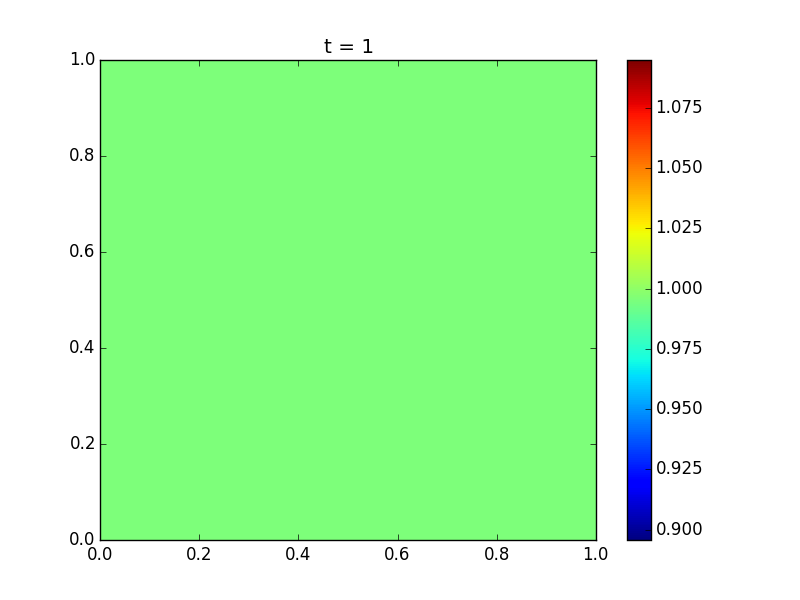
\includegraphics[scale=0.2]{img/slices2d/sl_1.png}
  \caption{$t = 1$ \label{fig1}}
 \end{minipage} \hfill
 \begin{minipage}[b]{.46\linewidth}
     \centering    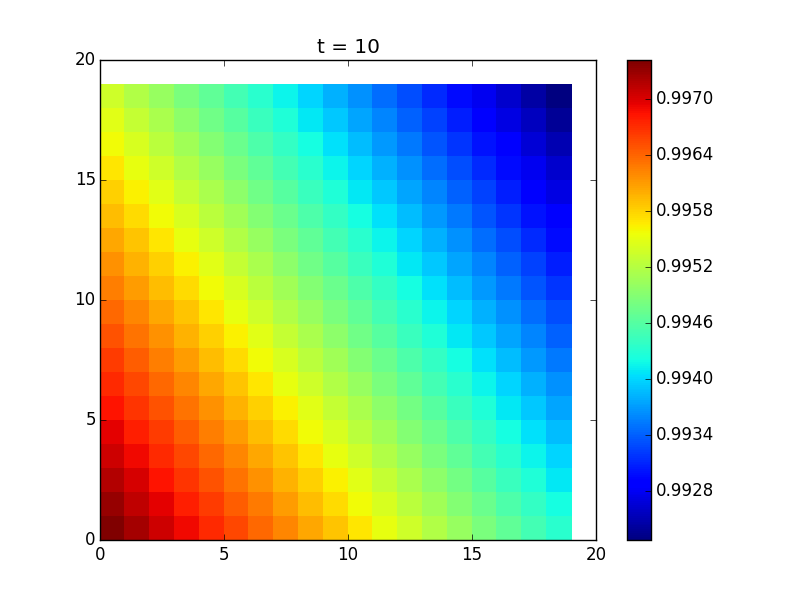
\includegraphics[scale=0.2]{img/slices2d/sl_10.png}
  \caption{$t = 10$ \label{fig2}}
\end{minipage}
 \begin{minipage}[b]{.46\linewidth}
     \centering    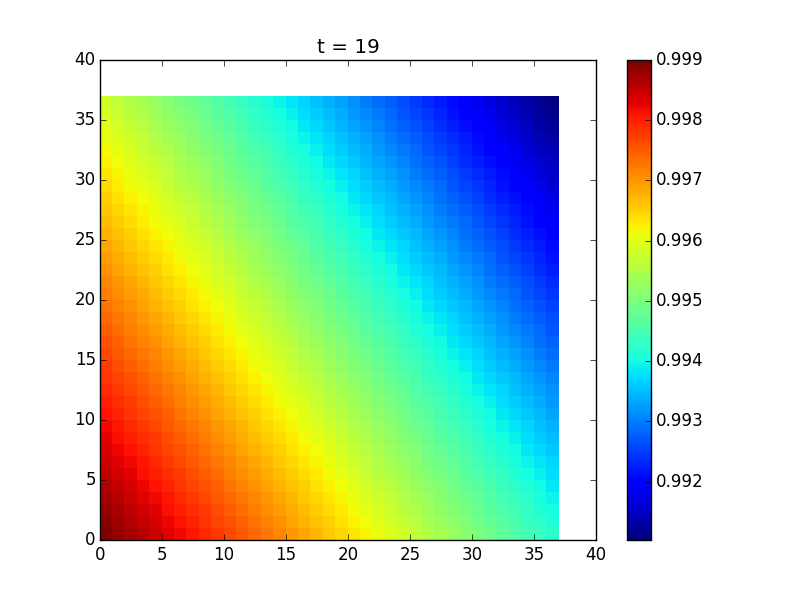
\includegraphics[scale=0.2]{img/slices2d/sl_19.png}
  \caption{$t = 20$ \label{fig3}}
\end{minipage}
 \begin{minipage}[b]{.46\linewidth}
     \centering    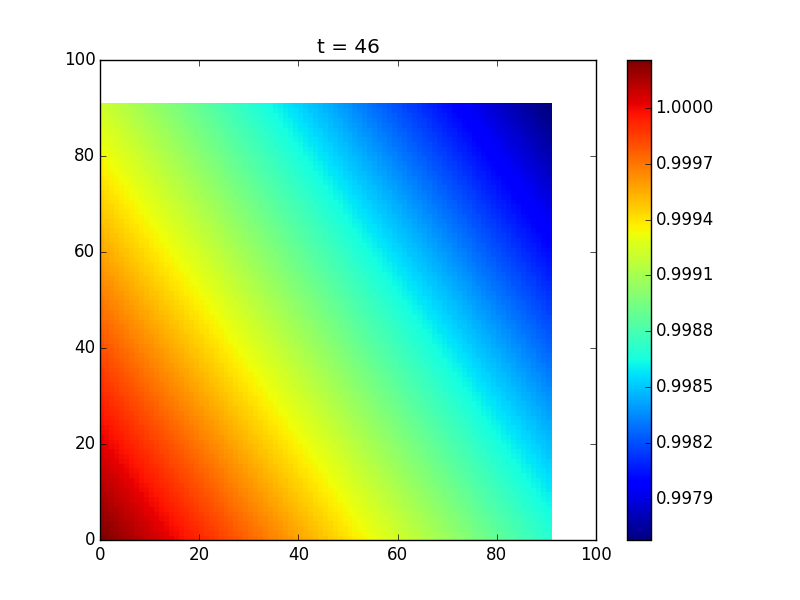
\includegraphics[scale=0.2]{img/slices2d/sl_46.png}
  \caption{$t = 30$}
\end{minipage}

\end{figure}

Une autre améliroation possible est de trouver une formule analytique pour certain produits. En effet, si nous reprenons l'exemple d'un cancellable spread option 2Y10Y dont la maturité est dans 5 ans, nous devrions normalement construite l'arbre jusqu'en 2030 pour avoir le taux 10Y en 2020. Nous pouvons éviter celà en fournissant directement une formule exacte pour les zéro coupons. C'est ce que nous faisons dans la partie suivante.

\subsection{Formule exacte}
Cette partie est fortement insipiré de \cite{Brugo}.

On rappelle l'expression du prix de l'obligation zéron coupon sous la mesure risque neutre $Q$
$$P(t, T) = \espr{ e^{-\int_t^T r_u \rm{d}u}} $$

Notons $I(t, T) := \int_t^T x(u) + y(u) \rm{d}u$, et montrons que conditionnellement à l'information accumulé jusqu'au temps $t$, que c'est une variable normale d'espérance $M(t, T)$ et de variance $V(t, T)$ où:
\begin{align}
  M(\beta^y, t, T) &:= \frac{1 - e^{-\beta^y (T-t) }}{\beta^y} \\
  V(\beta^y, \sigma^x, \beta^y, \sigma^y, t, T) &:= \frac{\sigma^x \sigma^y}{\beta^y \beta^y} \left[ T - t + \frac{e^{-\beta^y (T-t) } - 1}{\beta^y} + \frac{e^{-\beta^y (T-t) } - 1}{\beta^y} - \frac{e^{-(\beta^y + \beta^y) (T-t) } - 1}{\beta^y + \beta^y} \right] \\
  V(t, T) &:= V(\beta^y, \sigma^x, \beta^y, \sigma^x, t, T)
            + V(\beta^y, \sigma^y, \beta^y, \sigma^y, t, T)
            + 2 \rho V(\beta^y, \sigma^x, \beta^y, \sigma^y, t, T) \\
            M(t, T) &:= M(\beta^y, t, T) x(t) + M(\beta^y, t, T) y(t)
\end{align}

\begin{proof}
  Par simple calcul \cite{Brugo}:
  $$  \int_t^T x(u) \rm{d}u = \frac{1 - e^{-\beta^y (T-t)}}{\beta^y} + \frac{\sigma^x}{\beta^y} \int_t^T \left[1 - e^{-\beta^y (T-t)}\right] \rm{d} W^x_u$$
  $$  \espr{\int_t^T x(u) \rm{d}u} = M(\beta^y, t, T) x(t)$$
  $$ Var(\int_t^T x(u) \rm{d}u) =   \left(\frac{\sigma^x}{\beta^y}\right)^2 \espr{ \int_t^T \left[1 - e^{-\beta^y (T-t)}\right]^2 \rm{d}u } = V(\beta^y, \sigma^x, \beta^y, \sigma^x, t, T)$$ (isométrie d'itto)
\end{proof}

Nous avons donc
\begin{align}
  P(t, T) &= exp  \left(  -\int_t^T r_u \rm{d}u + \frac{1}{2} Var \left( {-\int_t^T r_u \rm{d}u} \right)  \right) \\
          &= exp  \left( - M(\beta^y, t, T) x(t) - M(\beta^y, t, T) y(t) + \frac{1}{2} V(t, T) \right)
  \end{align}

Nous utiliserons cette formule directement dans le pricer, ce qui nous évitera de construire l'arbre jusqu'à la date de maturité du dernier zéro coupon.

Pour mesurer l'impact de ce changement sur le temps d'execution du programme, nous avons utilisé le logiciel \textbf{valegrind}. Ce logiciel  permet le profilage du code, ie il permet de controler:
\begin{itemize}
\item la liste des fonctions appelées et le temps passé dans chacune d'elles
\item l'utilisation processepur
\item l'utilisation mémoire
\end{itemize}

Ci-dessous deux graphes produits par le logiciel qui illustre le nombre de fois que la fonction responsable de l'évolution de l'arbre \mintinline{cpp}{Hyb4_UpdateStatePricesOnly} est appelée:

\IMG{img/ycso2.png}{En utilisant l'arbre pour le calcul des $P(t, T)$}{0.5}
\IMG{img/ycso3.png}{En utilisant la formule exacte}{0.5}

Le nombre d'appels à cette fonction est environ réduit de moitié. Cette dernière étant très gourmande en ressource, le temps total requis par le programme est réduit de $~30\%$.

\subsection{Ajout d'un shift déterministe}
Le modèle, tel que développé jusqu'a présent, présente un inconvénient majeur: à tout instant, $r_t$ est symétriquement distribué autour de $0$. Ceci ne correspond pas à la réalité, puisque les taux négatifs ne sont observé dans les marchés que dans de très rares circonstance ( en Europe après crise inter-bancaire de 2009, Au Japon après des années de déflation ). Une autre raison est que le modèle ne permet pas de retrouver les prix des obligations zéro coupon.

Pour pallier à ce problème, nous rajoutons une fonction $\phi$ au taux $r_t$. La fonction déterministe $\phi(t)$ permet de fitter exactement la courbe de taux observée. Dans la partie ``Calibraion nous'' nous verrons comment calculer cette fonction à partir des prix de bonds zéro coupon.

En prenant en compte ce changement, le prix de l'obligation zéro coupon devient:

$$P(t, T) = \espr{ e^{-r_t + \phi(t)}}$$

Nous prendrons soin de modifier l'étape de ``draw back'' dans l'abre en changeant le facteur d'actualisation.

Le processus est markovien

\subsection{Optimiser la taille des slices }

La slice que nous avons construite est rectangulaire.
La plage que nous autorisons à $(x, y)$ doit logiquement dépendre de leur corrélation. Ainsi pour simuler deux processus parfaitement corrélés, il suffit de simuler l'un deux, la slice dans ce cas est simplement linéaire. Dans le cas ou ils sont indépendants, il est nécessaire de simuler les deux, et la slice sera parfaitement rectangulaire. Dans le cas général nous utilisons la méthode suivante 

Nous décomposons la source de stochasticité $dW_t$ en deux composantes indépendantes:
$$ \rm{d} W_t := (\rm{d} W^x_t, \rm{d} W^y_t)^T = A(t)  \rm{d}Z_t$$
où
$$
A(t) := 
\left(
  \begin{array}{cc}
            \sigma^x & 0  \\
            \rho \sigma^y & \sqrt{1-\rho^2} \sigma^y \  \\
  \end{array}
\right)
$$
$Z = (Z^1, Z^2)$ un mouvement brownien 2D à compostantes indépendantes.

A l'instant $t_n$,
$$x(t_{n+1}) := x_i(t_n) (1 - \beta^y \Delta) + ... Z_1$$
$$y(t_{n+1}) := y_i(t_n) (1 - \beta^y \Delta) + ... Z_1 + ...Z_2$$
Les limites de l'abre sont définie comme étant les bords de l'ellipsoid décrit par l'équation:

$$Z_1^2 + Z_2^2 \leq n_{\sigma^x}^2$$

Où $n_{\sigma^x}$ est sans unité et dénote le dégré de déviation de la moyenne qu'on autorise.


\subsection{ Paramètres dépendant du temps}

Dans la partie précédente, les paramètres ($\sigma^x, \sigma^y, \beta^y, \beta^y, \rho)$ étaient constantes. Pour plus de souplesse, nous considérons des variables qui dépendent  du temps, ou plus précisément constantes par morceaux.

Le calcul du prix des obligtions zéro coupon est fourni en annexe.

Deux problèmes cependant avec cette méthode:

\begin{itemize}
\item Le calcul est beaucoup plus long
\item possibilité de overfitter les données historique du marché, ce qui affecte négativement le pouvoir prédicitive du modèle
\end{itemize}


 


\chapter{Résultats}

Une fois toutes ces modifications prises en compte, nous pouvons 

\IMG{img/pending.jpg}{Slice 3D}{0.2}


\subsection{Performance}
L'arbre ainsi construit est puissant dans le sens où il permet de pricer quasiement tous les instruments dont on a besoin en pratique. Cependant ce modèle souffre de quelques défaut observé en pratique.

\begin{itemize}
\item  De par sa construction, l'arbre est bornée. Ce dernier ignore donc le comportement des driver loin de leurs moyenne. Si ceci n'est pas un problème dans le cadre de variable normale (poids centré), ceci peut engendrer des erreurs non négligeables quand les variables ont des distribution à queues épaisses.
\item  Discrétisation des processus
\item  probabilités négatives
\end{itemize}

Dans le cas des obligations zéro coupon, nous disposons d'une formule exacte pour calculer les prix et les comprarer à celles produites par l'arbre. 
Le schéma suivant montre la slice produite par l'arbre (brute force) et celle produite par la formule exacte (closed form) 
\IMG{img/slice.png}{Erreur bf vs cf Slice 3D}{0.7}

\chapter{Application: calibration et pricing}
Notre modèle possède à un certains nombres de paramètres libre que nous devons fixer. Pour celà, nous choisissons un certain nombre d'actifs tradables dans le marché, dont le prix est donc connus, que nous appelerons benchmark. Nous essayerons ensuite de trouver les paramètres qui reproduisent le mieux ces prix là. Cette procédure est appelé calibration.
Une question naturelle qui se pose est de savoir quels actifs choisir pour la calibration. Il existe plusieurs réponses possibles, en pratique on essaye de trouver un produit à la fois simple et liquide.

Dans notre cas il est indispensable que le modèle puissent retrouver les prix des bond zéro coupons.
Idéalement notre benchmarks est une ensemble de caplets. Les caplets ne sont pas tradés en tant que tel sur le marché, nous n'avons accès qu'à des caps. => Stripping

Le modèle à 2F permet de caputrer le hump de la courbe de rendement
Le nombre de paramètre est fini (5) => pas de overfitting


\begin{itemize}
\item $h(t)$ pour reconstruire la yield curve $\sigma \rho \nu$ pour
\item  matcher la surface
\end{itemize}

\subsection{Calibration du drift}
Le modèle gaussien à deux facteurs est calibré sur la
courbe $P^M (0, T ), T > 0$ de prix d’obligations zéro-coupon observés sur le
marché si et seulement si $\phi$ est définie par :
$$P^M(0, T) := e^{ \int_0^T \phi(s) \rm{d}s + M x(T) +M y(T) + \frac{1}{2} V}$$
Ce qui est équivalent à 
$$ \int_t^T \phi(s) \rm{d}s := \frac{P^M(0, T)}{P^M(0, t)} e^{-\frac{1}{2}(V(0, T) - V(0, t))}$$

Cependant, l’arbre ainsi simulé ne redonnera par exactement les prix des
obligations zéro-coupon $P^M(0, T_i)$. En effet, dans un arbre le taux simulé est
considéré constant sur la période $[T_i, T_{i+1}$, donc tout se passe comme
si l’arbre simulait en fait un taux zéro-coupon R. En d’autres termes, le prix
d’une obligation zéro-coupon de maturité $T_1$ vaut
$P(0, T_1 ) = e^{-R(0, T_1) \Delta t}$
mais ce prix calculé directement sur l’arbre s’écrira $e^{-r_0\Delta t}$ .
La figure ci-dessus illustre la différence entre les prix théorique et les prix calculés l'arbre:
\IMG{img/pending.jpg}{Diff Slice}{0.2}

On propose donc ici de calibrer récursivement les $\phi_i$ afin de
retrouver les prix des obligations zéro-coupon directement sur l’arbre. 
$\Pi_j$ state price (arrow debrew) (paye 1 si le noeud $(t_n, j)$ est atteint.

$$D_j(h_n) := \frac{1}{1 + r(t_n)(t_{n+1} - t_n)} $$ Le discount factor
$$ \Pi_j(t_{n+1}) = \sum_j \Pi_j(t_n) p_{j, j'}(t_n) D_{j'}(h_n)$$
$$ \sum \Pi_j D_j(h_n) = P(0, t_{n+1}) $$

Developement de taylor => trouver $h_n$

\subsection{Méthode de calibration de la surface - Méthode d'optimisation}

Les traders préfère aiment bien avoir un controle fin sur le modèle qui reflète leur sensation sur le marché. Pour celà, le modèle doit êtres paramètrble, les paramètres doivent avoir un sens/être compris par les traders.

Au lieu d'avoir un paramète par maturité, G2++ il y a 5 paramètres


\begin{itemize}
\item On s'autorise un intervalle pour les paramètres
\item On utilise une grille (définie par le pas) pour définir les valeurs
  autorisées pour chaque paramètre. (Tradeoff entre pas petite grande
  précision et temps de calculs)
\item On calcule le prix des caplets associés
\item On choisit les paramètre qui reflètent le mieux les prix du
  marché.
\end{itemize}

Maintenant que nous connaissons la dynamique de $P(t, T)$, nous pouvons fournir une formule explicite pour le prix des caplets.

En effet, sous la mesure forward neutre $Q_T$, l'equation vérifiér  par $(x, y)$ est:

\begin{align*}
  \rm{d}x &= -\alpha x(t) \rm{d}t - Drift_x + \sigma \rm{d}W^1_t \\
  \rm{d}y &= -\beta y(t) \rm{d}t - Drift_y + \nu \rm{d}W^2_t \\
\end{align*}

qui a donc pour solution:
\begin{align*}
  x(t) &= -\alpha x(t) \rm{d}t - Drift_x + \sigma \rm{d}W^1_t \\
  y(t) &= -\beta y(t) \rm{d}t - Drift_y + \nu \rm{d}W^2_t \\
\end{align*}

Nous rappeleons l'expression du caplet sour la mesure $Q_T$
$$ZBC = \Qespr{Q_T}{ ( } $$

$P(t, T)$ admet une distribution normale sous $Q_T$ conditionnellement à $F_t$, 
Le prix théorique:

$$ZBC(t, T, S, K) = -P(t, T) N( d_1 ) + P(t, T) K N(d_2)$$
$$d_{-+} := \frac{ln \frac{KP(t, T)}{P(t, S)}}{\Sigma} +- \frac{1}{2}\Sigma $$
$$\Sigma^2 := \Sigma^{x,x} + \Sigma^{y,y} + 2 \rho \Sigma^{x,y}$$
$$\Sigma^{x,y} := \sigma \nu M^x(t, T) M^y(t, T) \frac{1 - e^{(\alpha+\beta) (T-t)}}{\alpha+\beta} $$

On a 5 paramètres à optimiser
On calibre les caplets

Les caplets ne sont pas directement disponilbe sur les marche
On calibre les swaptions/caps

\begin{itemize}
\item Le probleme de calbration est un probleme d'optimisation Courbe
  de vol implicite :
\item minimisation de l'erreur L2
\end{itemize}
\IMG{img/capsurf.png}{Cap surface}{0.5}

\subsubsection{Un mot sur le multi threading - gpu?}
La méthode de calibration proposée ci-dessus à l'avantage d'être faciement paralélisable. Les calculs aux différents points de la grille sont indépendant.

%%% Local Variables:
%%% mode: latex
%%% TeX-master: "main"
%%% End:

\appendix

{\newgeometry{left=0.8in,right=0.8in,top=1in,bottom=1in}
\chapter{Code de simulation en Python}
\inputminted{python}{code/tree.py}
\chapter{Formule exacte des obligations zéro coupon pour des paramètres dépendant du temps}

Dans cette partie nous détaillerons le calcul de prix d'obligation zéro coupon dans le modèle de Hull-White à deux facteurs dans le cas où les paramètre sont dépendents du temps, ou plus précisément, constants par morceaux.

Le modèle est toujours markovien, c'est à dire que nous pouvons toujours écrire $P(t, T)$ comme une fonction détérministe de $(x(t), y(t)$:

$$P(t, T) := e^{\int_t^T \phi_s \rm{d}s - M_x(t, T) x(t) - M_y(t, T) y(t) + \frac{1}{2} V(t, T)}$$

Nous calculerons ici $M_x$, $M_y$ et $V$  

\subsection*{Rappel du modèle}
$$\rm{d}x_t = -\beta_x x_t \rm{d}t +  \sigma_x \rm{d} W^1_t $$
$$\rm{d}y_t = -\beta_y y_t \rm{d}t +  \sigma_y \rm{d} W^2_t $$
$$r_t =  \phi(t) + x_t  + y_t $$
$$\rho_t = <\rm{d} W^1_t, \rm{d} W^2_t>$$

\subsection*{Cas particulier: modèle à un seul facteur}
Nous commencerons par le cas particulier où $y(t) = 0$, l'équation différentielle vérifiée par $x(t)$ s'intègre facilement en:
$$x(t) = \sum_{t_i < t} \sigma_i  \int_{t_i}^{t \wedge t_{i+1}}  e^{- a (t \wedge t_{i+1}-s)}   \rm{d} W_1(s) $$

Nous devons maintenant intégrer la fonction $x$ entre $t_0$ et $t_f$ en la décomposant en somme d'intégrales entre les instant $t_i$ et $t_{i+1}$ où tous les paramètres sont constants et l'intégrale se calcule facilement.

\begin{align*}
\int_{t_0}^{t_f} x(t) dt &= \sum_i \int_{t_i}^{t_{i+1}} x(t) dt \\
&= \sum_i \frac{1 - e^{-\beta_i (t_{i+1} - t_i) }}{ \beta_i} x(t_i)
+ \frac{\sigma_i}{\beta_i} \int_{t_i}^{t_{i+1}} (1 - e^{-\beta_i (t_{i+1} - u)}) dW_u \\
&= \sum_i \frac{1 - e^{-\beta_i (t_{i+1} - t_i) }}{ \beta_i} e^{-\int_{t_0}^{t_i} \beta} x(t_0) \\
&+  \sum_i \frac{1 - e^{-\beta_i (t_{i+1} - t_i) }}{ \beta_i} \int_{t_0}^{t_i} \sigma_u e^{-\int_u^{t_i} \beta} dW_u
+ \frac{\sigma_i}{\beta_i} \int_{t_i}^{t_{i+1}} (1 - e^{-\beta_i (t_{i+1} - u)}) dW_u \\
&=: M(t_0, t_f) x(t_0) + v(t_0, t_f) \sim \mathcal{N}( M(t_0, t_f), V(t_0, t_f))
\end{align*}
où nous avons noté: $V(t_0, t_f) := Var( \int_{t_0}^{t_f} x ) = Var( v(t_0, t_f))$

d'où
\begin{align*}
P(t, T) &= E\left[ exp \left\{  -\int_t^T h(u) + E(-\int_t^T x) - \frac{1}{2} Var(-\int_t^T x) \!  \right\} \right]
\end{align*}

Simplifions l'écriture de $V(t_0, t_f)$
\begin{align*}
v(t_0,t_f) &:=
\sum_{i, t_0 \leq t_i \leq t_{i+1} \leq t_f }
\frac{1 - e^{-\beta_i (t_{i+1} - t_i) }}{ \beta_i} \int_{t_0}^{t_i} \sigma_u e^{-\int_u^{t_i} \beta} dW_u
+ \frac{\sigma_i}{\beta_i} \int_{t_i}^{t_{i+1}} (1 - e^{-\beta_i (t_{i+1} - u)}) dW_u \\
&=
\sum_{i}
\frac{1-e^{- \int_{t_i}^{t_{i+1}} \beta}}{\beta_i}
\int_{t}^{t_{i}} \sigma_u e^{-\int_u^{t_i} \beta} dW_u
+
\frac{\sigma_i}{\beta_i} \int_{t_i}^{t_{i+1}} 1-e^{-\int_u^{t_{i+1}} \beta} dWu  \\
&=
\int_{t_0}^{t_f} \frac{\sigma_u}{\beta_u} dW_u
+
\sum_{i }
\int_{t}^{t_{i}} \frac{\sigma_u}{\beta_i} e^{-\int_u^{t_i} \beta} dW_u
- \int_{t}^{t_{i}} \frac{\sigma_u}{\beta_i} e^{-\int_u^{t_{i+1}} \beta} dW_u
- \frac{\sigma_i}{\beta_i} \int_{t_i}^{t_{i+1}} e^{-\int_u^{t_{i+1}} \beta} du
\\
&=
\int_{t_0}^{t_f} \frac{\sigma_u}{\beta_u} dW_u
+
\sum_{i }
 \frac{ \int_{t}^{t_{i}}\sigma_u e^{-\int_u^{t_i} \beta} dW_u }{\beta_i}
- \frac{ \int_{t}^{t_{i+1}}\sigma_u e^{-\int_u^{t_{i+1}} \beta} dW_u}{\beta_i}
\\
&=
\int_{t_0}^{t_f} \frac{\sigma_u}{\beta_u} dW_u
+
\sum_{i}
\frac{K_i - K_{i+1}}{\beta_i}
& \text{with $K_i = \int_{t_0}^{t_{i}}\sigma_u e^{-\int_u^{t_i} \beta} dW_u $}
\\
&=
\int_{t_0}^{t_f} \frac{\sigma_u}{\beta_u} dW_u
+
\sum_{i}
(\frac{1}{\beta_i} - \frac{1}{\beta_{i+1}}) K_i\\
&=
\int_{t_0}^{t_f} \frac{\sigma_u}{\beta_u} dW_u
+
\sum_{i=1..n}c_i K_i
&\text{avec  $c_i = \frac{1}{\beta_i} - \frac{1}{\beta_{i-1}}$ and $\beta_{n} = \infty$}
\end{align*}

Nous sommes intéressés par la variance de cette quantité là:

\begin{align*}
Var(t_0, t_f) &:= var( v(t_0,t_f)| F_{t_0}  ) \\
&= <\int_{t_0}^{t_f} \frac{\sigma_u}{\beta_u} dW_u, \int_{t_0}^{t_f} \frac{\sigma_u}{\beta_u} dW_u>
+ 2 \sum_i c_i  < K_i , \int_{t_0}^{t_f} \frac{\sigma_u}{\beta_u} dW_u>
+  \sum_{i, j} c_i c_j <  K_i,   K_j> \\
&= \omega
+ 2 \sum_i c_i  \alpha_i
+  \sum_{i, j}c_i c_j \gamma_{ij} \\
&= \omega + 2 \sum_i c_i  \alpha_i
+  2 \sum_{i < j} c_i c_j e^{-\int_{t_i}^{t_j} \beta} \gamma_{i}
+ \sum_{i } c_i^2  \gamma_{i}
\\
&= \omega + 2 \sum_i c_i  \alpha_i
+ 2 \sum_{i=1..n} \gamma_{i} \frac{c_i}{I_i} \left( \sum_{j = i+1...n} I_j c_j \right)
+ \sum_{i } c_i^2  \gamma_{i}\\
&= \omega + 2 \sum_i c_i  \alpha_i
+ 2 \sum_{i=1..n} \gamma_{i} \frac{c_i}{I_i} \left( S_n - S_i \right)
+ \sum_{i } c_i^2  \gamma_{i}
\end{align*}

Où
\begin{align*}
  I_i &:= e^{-\int^{t_i}_0 \beta} \\
  S_i &:= \sum_{j = 0...i} I_j c_j \\
  \omega &:= \sum_i  (\frac{\sigma_i}{\beta_i})^2 (t_{i+1} - t_i)
\end{align*}

Et les suite $\alpha_i$ et $\gamma_i$ sont définies par réccurence:
  \begin{align*}
    \alpha_{i+1} &:= e^{-\beta_i (t_{i+1} - t_i)} \alpha_i + (\frac{\sigma_i}{\beta_i})^2 (1 - e^{-\beta_i(t_{i+1} - t_i)}) \\
    \gamma_{i+1} &:= e^{-2 \beta_i (t_{i+1} - t_i)} \gamma_i + \frac{\sigma_i^2}{2 \beta_i} (1 - e^{-2 \beta_i(t_{i+1} - t_i)})\\
\end{align*}
    
Dans la section suivante on détaille le calcul de $\alpha$, $\gamma$ et $\omega$

Cette formule permet de calculer $V$ en temps linéaire (ie $O(t_f - t_0)$)
\subsection*{Calculations}

Pour $i < j$
\begin{align*}
\gamma_{i, j} &:= <K_i, K_j>  \\
&= < \int_{t}^{t_i}\sigma_u e^{-\int_u^{t_i} \beta} dW_u,
\int_{t}^{t_j}\sigma_u e^{-\int_u^{t_j} \beta} dW_u > \\
&= e^{-\int_{t_i}^{t_j} \beta} \int_t^{t_i} (\sigma_u e^{-\int_u^{t_i} \beta})^2 du \\
&= e^{-\int_{t_i}^{t_j} \beta} \int_t^{t_i} \sigma_u^2 e^{-2 \int_u^{t_i} \beta} du \\
&= e^{-\int_{t_i}^{t_j} \beta} \gamma_{i, i}
\end{align*}

\begin{align*}
\gamma_{i+1} &:= \gamma_{i+1, i+1} \\
&= \int_t^{t_{i+1}} \sigma_u^2 e^{-2 \int_u^{t_{i+1}} \beta} du \\
&= e^{-2 \beta_i (t_{i+1} - t_i)} \gamma_i + \int_{t_i}^{t_{i+1}} \sigma_i^2 e^{-2 \beta_i(t_{i+1} - u)} du \\
&= e^{-2 \beta_i (t_{i+1} - t_i)} \gamma_i + \frac{\sigma_i^2}{2 \beta_i} (1 - e^{-2 \beta_i(t_{i+1} - t_i)})
\end{align*}

\begin{align*}
\alpha_i &:=
<K_i, \int_{t_0}^{t_f} \frac{\sigma_u}{\beta_u} dW_u> \\
&=
< \int_{t}^{t_i}\sigma_u e^{-\int_u^{t_i} \beta} dW_u,
\int_{t_0}^{t_f} \frac{\sigma_u}{\beta_u} dW_u > \\
&=   \int_t^{t_i} \frac{\sigma_u^2}{\beta_u} e^{-\int_u^{t_i} \beta} du \\
\end{align*}

\begin{align*}
\alpha_{i+1}
&= e^{-\beta_i (t_{i+1} - t_i)} \alpha_i + \int_{t_i}^{t_{i+1}} \frac{\sigma_u^2}{\beta_u} e^{-\beta_i(t_{i+1} - u)} du\\
&= e^{-\beta_i (t_{i+1} - t_i)} \alpha_i + (\frac{\sigma_i}{\beta_i})^2 (1 - e^{-\beta_i(t_{i+1} - t_i)})
\end{align*}


\begin{align*}
\omega &:=
<\int_{t_0}^{t_f} \frac{\sigma_u}{\beta_u} dW_u, \int_{t_0}^{t_f} \frac{\sigma_u}{\beta_u} dW_u>\\
&= \int_{t_0}^{t_f} (\frac{\sigma_u}{\beta_u})^2 du \\
&= \sum_i  (\frac{\sigma_i}{\beta_i})^2 (t_{i+1} - t_i)
\end{align*}

\subsection*{Le modèle à deux facteurs}
Nous revenons au modèle original à deux facteurs. Les paramètre relatifs au facteur $x$ (resp. $y$) seront dénoté par un x (resp. y) en exposant.

L'espérance étant linéaire, et la variance quadratique, 
$M(t_0, t_f)$ est remplacée par $M^x x + M^y y$, et $V(t_0, t_f)$ par $V^{xx} + V^{yy} + 2 V^{xy}$, de sorte que:

$$P(t_0, T_f) = exp(-\int_{t_0}^{t_f} \Phi - M^x(t_0, t_f) x(t_0) - M^y(t_0, t_f) y(t_0) + \frac{V(t_0, t_f)}{2})$$

\begin{align*} V^{xy} &:= <
\int_{t_0}^{t_f} \frac{\sigma^x_u}{\beta_u^x} dW_u^x+\sum_{i=1..n}c_i^x K_i^x,
\int_{t_0}^{t_f} \frac{\sigma^y_u}{\beta_u^y} dW_u^y+\sum_{i=1..n}c_i^y K_i^y> \\
&= \int_{t_0}^{t_f} \frac{\sigma_u^x \sigma_u^y}{\beta_u^x \beta_u^y} \rho_u du
+ \sum_{ij} c_i^x c_j^y <K_i^x, K_i^y>
+ \sum_i c_i^x <K_i^x \int_{t_0}^{t_f} \frac{\sigma^y_u}{\beta_u^y} dW_u^y> + c_i^y <K_i^y \int_{t_0}^{t_f} \frac{\sigma^x_u}{\beta_u^x} dW_u^x>\\
&= \omega^{x,y} + \sum_{ij} c_i^x c_j^y \gamma_{ij}^{xy}
+ \sum_i c_i^x \alpha_i^x + c_i^y \alpha_i^y
\end{align*}

avec comme pour le cas à un seul facteur:
$$\alpha^x_{i+1} = e^{-\beta^x_i(t_{i+1} - t_i)} \alpha^x_i + \rho_i \frac{\sigma^x_i \sigma^y_i}{\beta^x_i \beta^y_i} (1 - e^{-\beta^x_i(t_{i+1} - t_i)})$$
$$\gamma_{i+1} = e^{- (\beta^x_i+\beta^y_i) (t_{i+1} - t_i)} \gamma_i + \rho_i \frac{\sigma_i^x \sigma_i^y}{\beta_i^x + \beta_i^y} (1 - e^{- (\beta^x_i+\beta^y_i)(t_{i+1} - t_i)})$$
$$\omega := \sum_i \rho_i  \frac{\sigma_i^x \sigma_i^y}{\beta_i^x \beta_i^y} (t_{i+1} - t_i)$$

\iffalse
With $i \leq j$:
\begin{align*}
 \gamma_{ij}^{xy} &:= <K_i^x, K_i^y> \\
  &= <\int_t^{t_i} \sigma_u^x e^{-\int_t^{t_i} \beta^x} dW^x, \int_t^{t_j} \sigma_u^y e^{-\int_t^{t_j} \beta^y} dW^y> \\
  &= e^{-\int_{t_i}^{t_j} \beta_y} \int_t^{t_i} \sigma_u^x \sigma_u^y e^{-\int_t^{t_i} \beta^x + \beta_y} \rho_u du \\
&= e^{-\int_{t_i}^{t_j} \beta_y} \gamma_{ii}
\end{align*}
\fi






\end{document}


%%% Local Variables:
%%% mode: latex
%%% TeX-master: t
%%% End:
